%
% bessel.tex
%
% (c) 2021 Prof Dr Andreas Müller, OST Ostschweizer Fachhochschule
%
\section{Bessel-Funktionen
\label{buch:differntialgleichungen:section:bessel}}
\rhead{Bessel-Funktionen}
Die Besselsche Differentialgleichung
erlaubt Wellen mit zylindrischer
Symmetrie und die Strömung in einem zylindrischen Rohr zu beschreiben.
Die Auflösung eines optischen Systems wird durch die Beugung limitiert,
die Helligkeitskverteilung des Bildes einer Punktquelle ist
zylindersymmetrisch und kann mit Hilfe von Lösungen der Besselschen
Differentialgleichung beschrieben werden.
Die Besselsche Differentialgleichung hat im Allgemeinen keine Lösung,
die sich durch bekannte Funktionen ausdrücken lassen, es ist also
nötig, eine neue Familie von speziellen Funktionen zu definieren,
die Bessel-Funktionen.

%
% Besselsche Differentialgleichung
%
\subsection{Die Besselsche Differentialgleichung}
% XXX Wo taucht diese Gleichung auf
Die Besselsche Differentialgleichung ist die Differentialgleichung
\begin{equation}
x^2\frac{d^2y}{dx^2} + x\frac{dy}{dx} + (x^2-\alpha^2)y = 0
\label{buch:differentialgleichungen:eqn:bessel}
\end{equation}
\index{Differentialgleichung!Besselsche}%
\index{Besselsche Differentialgleichung}%
zweiter Ordnung
für eine auf dem Interval $[0,\infty)$ definierte Funktion $y(x)$.
Der Parameter $\alpha$ ist eine beliebige komplexe Zahl $\alpha\in \mathbb{C}$,
die Lösungsfunktionen hängen daher von $\alpha$ ab.

%
% Eigenwertproblem
%
\subsubsection{Eigenwertproblem}
Die Besselsche Differentialgleichung
\eqref{buch:differentialgleichungen:eqn:bessel}
kann man auch als Eigenwertproblem für den Bessel-Operator
\index{Bessel-Operator}%
\index{Operator!Bessel-}%
\begin{equation}
B = x^2\frac{d^2}{dx^2} + x\frac{d}{dx} + x^2
\label{buch:differentialgleichungen:bessel-operator}
\end{equation}
schreiben.
Eine Lösung $y(x)$ der Gleichung
\eqref{buch:differentialgleichungen:eqn:bessel}
erfüllt
\[
By
=
x^2y''+xy'+x^2y
=\alpha^2 y,
\]
ist also eine Eigenfunktion des Bessel-Operators zum Eigenwert
$\alpha^2$.

%
% Indexgleichung
%
\subsubsection{Indexgleichung}
Die Besselsche Differentialgleichung ist eine Differentialgleichung
der Art~\eqref{buch:differentialgleichungen:eqn:dglverallg} mit
\[
p(x) = 1
\qquad\text{und}\qquad
q(x) = x^2-\alpha^2.
\]
Nach den Ausführungen von
Abschnitt~\ref{buch:differentialgleichungen:subsection:verallgemeinrt},
muss die Lösung in der Form einer verallgemeinerten Potenzreihe 
gesucht werden.
Dazu muss zunächst die Indexgleichung
\[
0
=
X(X-1) + Xp_0 + q_0
=
X(X-1) + X - \alpha^2
=
X^2-\alpha^2
=
(X-\alpha)(X+\alpha)
\]
gelöst werden.
Die Nullstellen sind offenbar $\varrho_1=\alpha$ und $\varrho_2=-\alpha$.

Die beiden Vorzeichen der Nullstellen der Indexgleichung führen
auf die gleiche Differentialgleichung.
Der Lösungsraum der Differentialgleichung ist natürlich trotzdem
zweidimensional, so dass es immer noch möglich ist, den
beiden Nullstellen der Indexgleichung verschiedene Lösungen
zuzuordnen.
Die Diskussion in
Abschnitt~\ref{buch:differentialgleichungen:subsection:verallgemeinrt}
hat Kriterien ergeben, unter denen zwei linear unabhängige Lösungen
mit Hilfe einer verallgemeinerten Potenzreihe gefunden werden können.
Falls nur eine solche Lösung gefunden werden kann, wird sie der grösseren
der beiden Zahlen $\alpha$ und $-\alpha$ zugeordnet
(oder $0$, falls $\alpha=-\alpha=0$).
Eine weitere Lösung kann mit Hilfe analytischer Fortsetzung gefunden werden,
wie später gezeigt wird.

Für nicht reelles $\alpha$ kann $\varrho_1-\varrho_2=2\alpha$ keine 
Ganzzahl sein, es ist also garantiert, dass zwei linear unabhängig
Lösungen der Form
\begin{equation}
y_1(x) = x^\alpha\sum_{k=0}^\infty a_kx^k
\qquad\text{und}\qquad
y_2(x) = x^{-\alpha}\sum_{k=0}^\infty b_kx^k.
\label{buch:differentialgleichungen:eqn:besselloesungen}
\end{equation}
existieren.

Für reelles $\alpha\in\mathbb{R}$ gibt es zwei Lösungen der
Form~\eqref{buch:differentialgleichungen:eqn:besselloesungen}
genau dann, wenn $\varrho_1-\varrho_2$ keine Ganzzahl ist.
Nur eine Lösung kann man finden, wenn 
\[
\alpha-(-\alpha)=2\alpha \in \mathbb{Z}
\qquad\Rightarrow\qquad
\alpha = \frac{k}{2},\quad k\in\mathbb{Z}
\]
ist.

%
% Bessel-Funktionen erster Art
%
\subsection{Bessel-Funktionen erster Art
\label{buch:differentialgleichungen:subsection:bessel1steart}}
Für $\alpha \ge 0$ gibt es immer mindestens eine Lösung der Besselgleichung
als verallgemeinerte Potenzreihe mit $\varrho=\alpha$.
Die Funktion $q(x)=x^2-\alpha^2$ ist ein Polynom, die einzigen
von $0$ verschiedenen Koeffizienten sind $q_0=-\alpha^2$
und $q_2=1$.
Für den ersten Koeffizienten $a_0$ gibt es keine Einschränkungen,
wir wählen $a_0=1$.

Die Rekursionsformel für $n=1$ ist
\[
F(\varrho+1) a_1 = (\varrho p_1+q_1)a_0,
\]
aber die Koeffizienten $p_1$ und $q_1$ verschwinden beide und damit
die ganze rechte Seite.
Da $F(\varrho+1)\ne 0$ ist, folgt dass $a_1=0$ sein muss.

% Fall n=1 gesondert behandeln

%
% Der allgemeine Fall
%
\subsubsection{Der allgemeine Fall}
Für die höheren Potenzen $n>1$ wird die Rekursionsformel für die
Koeffizienten $a_n$ der verallgemeinerten Potenzreihe
\[
a_{n} =
-\frac{ q_2 a_{n-2} }{F(\varrho+n)}
=
-\frac{a_{n-2}}{(\varrho+n)^2-\alpha^2}
=
-\frac{a_{n-2}}{\varrho^2 + 2\varrho n+n^2-\alpha^2}
=
-\frac{a_{n-2}}{n(n+2\varrho)}.
\]
Im letzten Schritt haben wir verwendet, dass $\varrho=\pm\alpha$
und damit $\varrho^2=\alpha^2$ ist.
Daraus folgt wegen $a_1=0$, dass auch $a_{2k+1}=0$ für alle $k$.
Damit können wir jetzt die Reihe hinschreiben:
\begin{align*}
y(x)
&=
x^{\varrho}\biggl(
1
-
\frac{1}{2(2+2\varrho)} x^2
+
\frac{1}{2(2+2\varrho)4(4+2\varrho)} x^4
-
\frac{1}{2(2+2\varrho)4(4+2\varrho)6(6+2\varrho)} x^6
+
\dots
\biggr)
\\
&=
x^{\varrho}
\biggl(
1
+
\frac{(-x^2/4)}{1\cdot (1+\varrho)}
+
\frac{(-x^2/4)^2}{1\cdot 2\cdot (1+\varrho)\cdot(2-\varrho)}
+
\frac{(-x^2/4)^3}{1\cdot 2\cdot 3\cdot (1+\varrho)\cdot(2+\varrho)\cdot(3+\varrho)}
+
\dots
\biggr)
\\
&=
x^\varrho\biggl(
1
+
\frac{1}{(\varrho+1)}\frac{(-x^2/4)}{1!}
+
\frac{1}{(\varrho+1)(\varrho+2)}\frac{(-x^2/4)^2}{2!}
+
\frac{1}{(\varrho+1)(\varrho+2)(\varrho+3)}\frac{(-x^2/4)^3}{3!}
+
\dots
\biggr)
\\
&=
x^\varrho \sum_{k=0}^\infty
\frac{1}{(\varrho+1)_k} \frac{(-x^2/4)}{k!}
=
x^\varrho
\cdot
\mathstrut_0F_1\biggl(;\varrho+1;-\frac{x^2}{4}\biggr)
\end{align*}
Wir finden also zwei Lösungsfunktionen
\begin{align}
y_1(x)
%J_\alpha(x)
&=
x^{\alpha\phantom{-}}
\sum_{k=0}^\infty
\frac{1}{(\alpha+1)_k}
\frac{(-x^2/4)^k}{k!}
=
x^\alpha
\cdot
\mathstrut_0F_1\biggl(;\alpha+1;-\frac{x^2}{4}\biggr),
\label{buch:differentialgleichunge:bessel:eqn:erste}
\\
y_2(x)
%J_{-\alpha}(x)
&=
x^{-\alpha} \sum_{k=0}^\infty
\frac{1}{(-\alpha+1)_k} \frac{(-x^2/4)^k}{k!}
=
x^{-\alpha}
\cdot
\mathstrut_0F_1\biggl(;-\alpha+1;-\frac{x^2}{4}\biggr).
\label{buch:differentialgleichunge:bessel:eqn:zweite}
\end{align}
Man beachte, dass die zweite Lösung für ganzzahliges $\alpha>0$ nicht
definiert ist.
Man kann auch direkt nachrechnen, dass diese Funktionen Lösungen
der Besselschen Differentialgleichung sind.

%
% Bessel-Funktionen
%
\subsubsection{Bessel-Funktionen}
Da die Besselsche Differentialgleichung linear ist, ist auch
jede Linearkombination der Funktionen
\eqref{buch:differentialgleichunge:bessel:eqn:erste}
und
\eqref{buch:differentialgleichunge:bessel:eqn:zweite}
eine Lösung.
Satz~\ref{buch:rekursion:gamma:satz:gamma-pochhammer}
ermöglicht, das Pochhammer-Symbol durch Werte der Gamma-Funktion
wie in
\[
(\alpha+1)_n = \frac{\Gamma(\alpha+k+1)}{\Gamma(\alpha+1)}
\]
auszudrücken.
Damit wird
\begin{align}
y_1(x)
&=
x^\alpha
\sum_{k=0}^\infty
\frac{\Gamma(\alpha+1)}{\Gamma(\alpha+k+1)}
\frac{(-x^2/4)^k}{k!}
=
\Gamma(\alpha+1) 2^{\alpha}
\biggl(\frac{x}{2}\biggr)^\alpha
\sum_{k=0}^\infty
\frac{(-1)^k}{k!\,\Gamma(\alpha+k+1)} \biggl(\frac{x}{2}\biggr)^{2k}
\label{buch:differentialgleichungen:bessel:normierungsgleichung}
\end{align}
Nur gerade der Faktor $2^\alpha\Gamma(\alpha+1)$ ist von $k$ und $x$ 
unabhängig, daher ist die folgende Definition sinnvoll:

\begin{definition}
\label{buch:differentialgleichungen:bessel:definition}
Die Funktion
\[
J_{\alpha}(x)
=
\biggl(\frac{x}{2}\biggr)^\alpha
\sum_{k=0}^\infty
\frac{(-1)^k}{k!\,\Gamma(\alpha+k+1)}
\biggl(\frac{x}{2}\biggr)^{2k}
\]
heisst {\em Bessel-Funktion erster Art der Ordnung $\alpha$}.
\index{Bessel-Funktion!erster Art}%
\end{definition}

Die Bessel-Funktion $J_\alpha(x)$ der Ordnung $\alpha$ unterscheidet sich
nur durch einen Normierungsfaktor von der Lösung $y_1(x)$.
Dasselbe gilt für $J_{-\alpha}(x)$ und $y_2(x)$:
\begin{align*}
J_{\alpha}(x)
&=
\frac{1}{2^\alpha\Gamma(\alpha+1)}
\cdot
y_1(x)
\\
J_{-\alpha}(x)
&=
\frac{1}{2^{-\alpha}\Gamma(-\alpha+1)}
\cdot
y_2(x).
\end{align*}

%
% Ganzzahlige Ordnung
%
\subsubsection{Besselfunktionen ganzzahliger Ordnung}
Man beachte, dass diese Definition für beliebige ganzzahlige 
$\alpha$ funktioniert.
Ist $\alpha=-n<0$, $n\in\mathbb{N}$, dann hat der Nenner Pole 
an den Stellen $k=0,1,\dots,n-1$.
Die Summe beginnt also erst bei $k=n$ oder
\begin{align*}
J_{-n}(x)
&=
\sum_{k=n}^\infty \frac{(-1)^k}{m!\,k!}\biggl(\frac{x}{2}\biggr)^{2k-n}
=
\sum_{l=0}^\infty
\frac{(-1)^{l+n}}{m!\,(l+n)!}\biggl(\frac{x}{2}\biggr)^{2(l+n)-n}
=
(-1)^n
\sum_{l=0}^\infty
\frac{(-1)^l}{m!\,\Gamma(l+n+1)}\biggl(\frac{x}{2}\biggr)^{2l+n}
\\
&=
(-1)^n
J_{n}(x).
\end{align*}
Insbesondere unterscheiden sich $J_n(x)$ und $J_{-n}(x)$ nur durch
ein Vorzeichen.

Als lineare Differentialgleichung zweiter Ordnung erwarten wir noch
eine zweite, linear unabhängige Lösung.
Diese kann jedoch nicht allein mit der Potenzreihenmethode,
dazu sind die Methoden der Funktionentheorie nötig.
Im Abschnitt~\ref{buch:funktionentheorie:subsection:dglsing}
wird gezeigt, wie dies möglich ist und auf
Seite~\pageref{buch:funktionentheorie:subsubsection:bessel2art}
werden die damit zu findenden Bessel-Funktionen 0-ter Ordnung und
zweiter Art vorgestellt.

%
% Erzeugende Funktione
%
\subsubsection{Erzeugende Funktion}
\begin{figure}
\centering
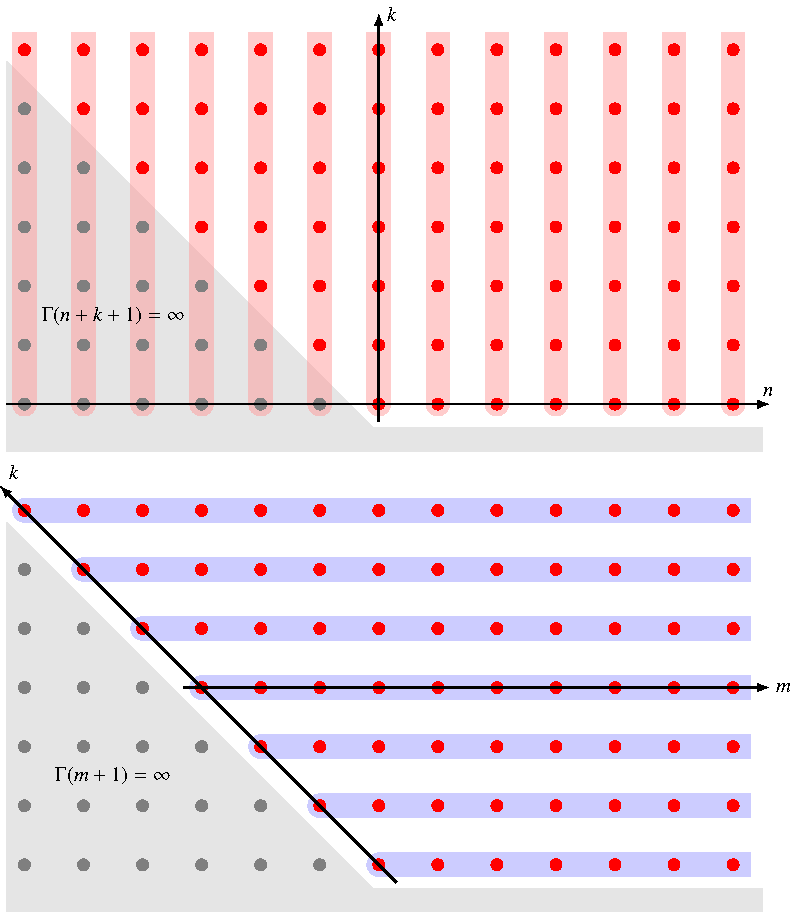
\includegraphics{chapters/050-differential/images/besselgrid.pdf}
\caption{Indexmenge für Herleitung der erzeugenden Funktion der
Besselfunktionen.
Die rote Summe in \eqref{buch:differentialgleichungen:bessel:eqn:rotesumme}
entspricht den vertikalen roten Streifen oben,
die blaue Summe in
\eqref{buch:differentialgleichungen:bessel:eqn:blauesumme}
den horizontalen Streifen in der Abbildung unten.
Alle Terme enthalten $\Gamma(n+k+1)$ im Nenner,
im grau hinterlegten Gebiet verschwinden sie.
\label{buch:differentialgleichungen:bessel:fig:indexmenge}}
\end{figure}
Die erzeugende Funktion der Bessel-Funktionen ist die Summe
\begin{align}
\sum_{n\in\mathbb{Z}} J_n(x)z^n
&=
\sum_{n\in\mathbb{Z}}
{\color{darkred}
\sum_{k=0}^\infty
\frac{(-1)^k}{k!\,\Gamma(k+n+1)}
\biggl(\frac{x}{2}\biggr)^{2k+n}
}
z^n.
\label{buch:differentialgleichungen:bessel:eqn:rotesumme}
\intertext{Die rote Summe entspricht den vertikalen roten Streifen in
Abbildung~\ref{buch:differentialgleichungen:bessel:fig:indexmenge} oben.
Die grau hinterlegten Punkte in der Abbildung gehören zu verschwindenden
Termen.
Wir schreiben $m=k+n$ und drücken alle Terme durch $k$ und $m$ aus:}
&=
\sum_{n\in \mathbb{Z}}
\sum_{k=0}^\infty
\frac{(-1)^k}{k!\,\Gamma(n+k+1)}
\biggl(\frac{x}{2}\biggr)^k
\biggl(\frac{x}{2}\biggr)^{n+k}
z^{n+k}
z^{-k}
\notag
\\
&=
\sum_{m\in \mathbb{Z}}
\sum_{k=0}^\infty \frac{(-1)^k}{k!}
\biggl(\frac{x}{2}\biggr)^k
z^{-k}
\frac{1}{\Gamma(m+1)}
\biggl(\frac{x}{2}\biggr)^{m}
z^{n+k}
\notag
\intertext{Auch in dieser Summe fallen wieder die Terme mit $m<0$
wegen $\Gamma(m+1)=\infty$ weg.
Die Grenzen der Summation über $k$ hängen nicht von $m$ ab, daher
können wir die Summationsreihenfolge vertauschen.
Die Summation über $m$ entspricht den horizontalen blauen Streifen
in 
Abbildung~\ref{buch:differentialgleichungen:bessel:fig:indexmenge}
unten.
Es ergibt sich die Summe}
&=
\sum_{k=0}^\infty
\sum_{m=0}^\infty
\frac{(-1)^k}{k!}
\biggl(\frac{x}{2}\biggr)^k
z^{-k}
\frac{1}{\Gamma(m+1)}
\biggl(\frac{x}{2}\biggr)^{m}
z^{m}
\notag
\\
&=
\sum_{k=0}^\infty \frac{(-1)^k}{k!}
\biggl(\frac{x}{2}\biggr)^k
z^{-k}
\cdot
{\color{blue}
\sum_{m=0}^\infty
\frac{1}{\Gamma(m+1)}
\biggl(\frac{x}{2}\biggr)^{m}
z^{m}
}.
\label{buch:differentialgleichungen:bessel:eqn:blauesumme}
\intertext{Beide Reihen sind Exponentialreihen, was man besser sehen kann,
wenn man die Gamma-Funktion in der zweiten Summe wieder als die
Fakultät $\Gamma(m+1)=m!$ schreibt.
Die beiden Exponentialreihen sind
}
&=
\sum_{k=0}^\infty \frac{\bigl(-\frac{x}2\cdot\frac1z\bigr)}{k!}
\cdot
\sum_{m=0}^\infty
\frac{\bigl(z\frac{x}2\bigr)^m}{m!}
=
\exp\biggl(\frac{x}2\cdot\biggl(-\frac1z\biggr)\biggr)
\cdot
\exp\biggl(\frac{x}2\cdot z\biggr)
=
\exp\biggl(\frac{x}2\cdot\biggl(z-\frac1z\biggr)\biggr).
\notag
\end{align}

%
% Additionstheorem
%
\subsubsection{Additionstheorem}
Die erzeugende Funktion kann dazu verwendet werden, das Additionstheorem
für die Besselfunktionen zu beweisen.

\begin{satz}
\index{Satz!Additionstheorem für Besselfunktionen}%
Für $l\in\mathbb{Z}$ und $x,y\in\mathbb{R}$ gilt
\[
J_l(x+y) = \sum_{m=-\infty}^\infty J_m(x)J_{l-m}(y).
\]
\end{satz}

\begin{proof}[Beweis]
Die Koeffizienten der erzeugenden Funktion der Bessel-Funktionen für
das Argument $x+y$ ist
\begin{align*}
\exp\biggl(\frac{x+y}2\biggl(z+\frac1z\biggr)\biggr)
&=
\sum_{n=-\infty}^\infty J_n(x+y)z^n.
\intertext{%
Wir verwenden die Exponentialgesetze auf der linken Seite und 
erhalten}
&=
\exp\biggl(\frac{x}2\biggl(z+\frac1z\biggr)\biggr)
\cdot
\exp\biggl(\frac{y}2\biggl(z+\frac1z\biggr)\biggr).
\intertext{Beide Faktoren sind erzeugende Funktionen von Bessel-Funktionen,
wir können sie also als}
&=
\sum_{m=-\infty}^\infty J_m(x)z^m
\cdot
\sum_{k=-\infty}^\infty J_k(y)z^k
\intertext{schreiben.
Durch Ausmultiplizieren und Zusammenfassen von Termen mit gleichem
Exponenten finden wir
}
&=
\sum_{m,k} J_m(x)J_k(y) z^{k+m}
=
\sum_{l=-\infty}^\infty
\biggl(
\sum_{m=-\infty}^\infty J_m(x)J_{l-m}(y)
\biggr)
z^l.
\intertext{Daraus folgt schliesslich mit Koeffizientenvergleich das
Additionstheorem}
J_l(x+y) &= \sum_{m=-\infty}^\infty J_m(x)J_{l-m}(y)
\end{align*}
für alle $l$.
\end{proof}

%
% Der Fall \alpha=0
% 
\subsubsection{Der Fall $\alpha=0$}
Im Fall $\alpha=0$ hat das Indexpolynom eine doppelte Nullstelle, wir
können daher nur eine Lösung erwarten.
Im Fall $\alpha=0$ wird das Produkt im Nenner zu $n!$, so dass die
Lösungsfunktion
\[
J_0(x)
=
\sum_{k=0}^\infty
\frac{(-1)^k}{(k!)^2}
\biggl(\frac{x}{2}\biggr)^{2k}
\]
geschrieben werden kann.


%
% Der Fall \alpha=p, p\in \mathbb{N}
%
\subsubsection{Der Fall $\alpha=p$, $p\in\mathbb{N}, p > 0$}
In diesem Fall kann nur die erste
Lösung~\eqref{buch:differentialgleichunge:bessel:erste}
verwendet werden.
Damit erhält die Lösungsfunktion die Form
\[
J_p(x)
=
\sum_{k=0}^\infty
\frac{(-1)^k}{k!(p+k)!}\biggl(\frac{x}{2}\biggr)^{p+2k}.
\]

%
% Der Fall $\alpha=n+\frac12$
%
\subsubsection{Der Fall $\alpha=n+\frac12$, $n\in\mathbb{N}$}
Obwohl $2\alpha$ eine Ganzzahl ist, sind die beiden Lösungen
\label{buch:differentialgleichunge:bessel:erste}
und
\label{buch:differentialgleichunge:bessel:zweite}
linear unabhängig.

Man kann zeigen, dass sich die Lösungsfunktionen in diesem Fall
durch bereits bekannte elementare Funktionen ausdrücken lassen.
Wir rechnen dies für $n=0$ nach.
Zunächst drücken wir die Pochhammer-Symbole im Nenner anders aus.
Es ist
\begin{align*}
\biggl(\frac12 + 1\biggr)_k
&=
\biggl(\frac12 + 1\biggr)
\biggl(\frac12 + 2\biggr)
\cdots
\biggl(\frac12 + k\biggr)
=
\frac{1}{2^k}\bigl(3\cdot 5\cdot\ldots\cdot (2k+1)\bigr)
=
\frac{(2k+1)!}{2^{2k}\cdot k!}
\\
\biggl(-\frac12 + 1\biggr)_k
&=
\biggl(-\frac12 + 1\biggr)
\biggl(-\frac12 + 2\biggr)
\cdots
\biggl(-\frac12 + k\biggr)
\\
&=
\biggl(\frac12 + 0\biggr)
\biggl(\frac12 + 1\biggr)
\cdots
\biggl(\frac12 + k-1\biggr)
=
\frac{1}{2^k}\bigl(1\cdot 3 \cdot\ldots\cdot (2(k-1)+1)\bigr)
=
\frac{(2k-1)!}{2^{2k-1}\cdot (k-1)!}
\end{align*}
Damit können jetzt die Reihenentwicklungen der Lösung wie folgt
umgeformt werden
\begin{align*}
y_1(x)
&=
x^\alpha
\sum_{k=0}^\infty
\frac{1}{(\alpha+1)_k}
\frac{(-x^2/4)^k}{k!}
=
\sqrt{x}
\sum_{k=0}^\infty
\frac{2^{2k}k!}{(2k+1)!}
\frac{(-x^2/4)^k}{k!}
=
\sqrt{x}
\sum_{k=0}^\infty
(-1)^k
\frac{x^{2k}}{(2k+1)!}
\\
&=
\frac{1}{\sqrt{x}}
\sum_{k=0}^\infty
(-1)^k
\frac{x^{2k+1}}{(2k+1)!}
=
\frac{1}{\sqrt{x}} \sin x
\\
y_2(x)
&=
x^{-\alpha}
\sum_{k=0}^\infty
\frac{1}{(-\alpha+1)_k}
\frac{(-x^2/4)^k}{k!}
=
x^{-\frac12}
\sum_{k=0}^\infty
\frac{2^{2k-1}\cdot (k-1)!}{(2k-1)!}
\frac{(-x^2/4)^k}{k!}
\\
&=
\frac{1}{\sqrt{x}}
\sum_{k=0}^\infty
(-1)^k
\frac{x^{2k}}{(2k-1)!\cdot 2k}
=
\frac{1}{\sqrt{x}} \cos x.
\end{align*}

Die Bessel-Funktionen verwenden aber eine andere Normierung. 
Die Gleichung~\eqref{buch:differentialgleichungen:bessel:normierungsgleichung}
zeigt, dass die Bessel-Funktionen durch Division
der Funktion $y_1(x)$ und $y_2(x)$ durch $2^\alpha \Gamma(\alpha+1)$ 
erhalten werden können.
Dies ergibt
\begin{equation*}
\renewcommand{\arraycolsep}{1pt}
\begin{array}{rclclclcl}
J_{\frac12}(x)
&=&
\displaystyle\frac{1}{2^{\frac12}\Gamma(\frac12+1)}
y_1(x)
&=&
\displaystyle\frac{1}{2^{\frac12}\frac12\Gamma(\frac12)}
y_1(x)
&=&
\displaystyle\frac{\sqrt{2}}{\Gamma(\frac12)}
y_1(x)
&=&
\displaystyle\frac{1}{\Gamma(\frac12)}
\sqrt{ \frac{2}{x}}
\sin x,
\\
J_{-\frac12}(x)
&=&
\displaystyle\frac{1}{2^{-\frac12}\Gamma(-\frac12+1)}
y_2(x)
&=&
\displaystyle\frac{2^{\frac12}}{\Gamma(\frac12)}
y_2(x)
&=&
\displaystyle\frac{\sqrt{2}}{\Gamma(\frac12)}
y_2(x)
&=&
\displaystyle\frac{1}{\Gamma(\frac12)}
\sqrt{\frac{2}{x}}
\cos x.
\end{array}
\end{equation*}
Wegen $\Gamma(\frac12)=\sqrt{\pi}$ sind die
halbzahligen Bessel-Funktionen daher
\begin{align*}
J_{\frac12}(x)
&=
\sqrt{\frac{2}{\pi x}} \sin x
=
\sqrt{\frac{2}{\pi}} x^{-\frac12}\sin x
&
&\text{und}&
J_{-\frac12}(x)
&=
\sqrt{\frac{2}{\pi x}} \cos x
=
\sqrt{\frac{2}{\pi}} x^{-\frac12}\cos x.
\end{align*}

%
% Direkte Verifikation der Lösungen
%
\subsubsection{Direkte Verifikation der Lösungen für $\alpha=\pm\frac12$}
Tatsächlich führt die Anwendung des Bessel-Operators auf die beiden
Funktionen auf
\begin{align*}
\sqrt{\frac{\pi}2}
BJ_{\frac12}(x)
&=
\sqrt{\frac{\pi}2}
\biggl(
x^2J_{\frac12}''(x) + xJ_{\frac12}'(x) + x^2J_{\frac12}(x)
\biggr)
\\
&=
x^2(x^{-\frac12}\sin x)''
+
x(x^{-\frac12}\sin x)'
+
x^2(x^{-\frac12}\sin x)
\\
&=
x^2(
x^{-{\textstyle\frac12}}\cos x
-{\textstyle\frac12}x^{-\frac32}\sin x
)'
+
x(
x^{-\frac12}\cos x
-{\textstyle\frac12}x^{-\frac32}\sin x
)
+
x^{\frac32}\sin x
\\
&=
x^2(
-x^{-\frac12}\sin x
-{\textstyle\frac12}x^{-\frac32}\cos x
-{\textstyle\frac12}x^{-\frac32}\cos x
+{\textstyle\frac{3}{4}}x^{-\frac52}\sin x
)
+
x^{\frac12}\cos x
+
x^{-\frac12}(x-{\textstyle\frac12})\sin x
\\
&=
(
-x^{\frac32}
+{\textstyle\frac34}x^{-\frac12}
+x^{\frac32}
-{\textstyle\frac12}x^{-\frac12}
)
\sin x
=
\frac14x^{-\frac12}\sin x
=
\frac14
\sqrt{\frac{\pi}2}
J_{\frac12}(x)
\\
BJ_{\frac12}(x)
&=
\biggl(\frac12\biggr)^2 J_{\frac12}(x).
\end{align*}
Dies zeigt, dass $J_{\frac12}(x)$ tatsächlich eine Eigenfunktion
des Bessel-Operators zum Eigenwert $\alpha^2 = \frac14$ ist.
Analog kann man die Lösung $y_2(x)$ für $-\frac12$ verifizieren.

